
\providecommand{\myrootdir}{..}
\documentclass[\myrootdir/main.tex]{subfiles}

\begin{document}

\chapter{The Failing Build Logs Data Set}
\includegraphics[page=5, width=\textwidth, trim={0.5cm 0.5cm 0.5cm 0.5cm}, clip]{img/flow-of-research.pdf}

\label{data-set}
\section{Motivation}
originally: log collection to get impression of build logs from various projects, what possibly extractable information they contain and how strutured or unstructured they are.
Then labeling of one build log information, namely the reason the build failed, as well as keywords and stuructural category to use in our evaluation and support our impressions about suitability of the techniques with quantitative results

\section{Log Collector}
ghtorrent, travis, implementation description, reference CLI interface nicely?
describe special cases?
\todo{image! like in travistorrent paper}

\section{Collection Process}
differentiate original collection and for data set?
actual instantiation: 30 langs, 3 repos that use Travis, 10 failed logs each -> 80 useable, x logs
our impression?
\todo{image!}

\section{Labeling (better name?)}
  \subsection{Build Failure Reason}

    \paragraph{Description}
    WHY? one common information developers and researches might want to extract, intentionally not focus on one structurally clearly defined extraction   cause that would be simple for PROSE extraction -> better comparability
    \paragraph{Labeling Process}

  \subsection{Keywords}

    \paragraph{Description}

    \paragraph{Labeling Process}

  \subsection{Categories}

    \paragraph{Description}

    \paragraph{Labeling Process}

\section{Validation of our data set}
\todo{copy over from md doc}

\subsection{Inter-Rater Reliability}

\subsection{Sending Mails out to developers}

\end{document}
